% !TEX root = ../main.tex

\section{Synthetic Shortcuts to Control Shared Information}
\label{eval:method}

In Section~\ref{sec:background} we show the suboptimality of the contrastive InfoNCE loss with multiple captions per image.
In the case of real-world \ac{VL} datasets with multiple captions per image, there are no annotations that indicate the information shared between the image and captions and the information specific to each caption.
Hence, we cannot directly measure how much of the shared and unique information is captured by the representations.

\begin{wrapfigure}[17]{R}{0.4\textwidth}
	\centering
	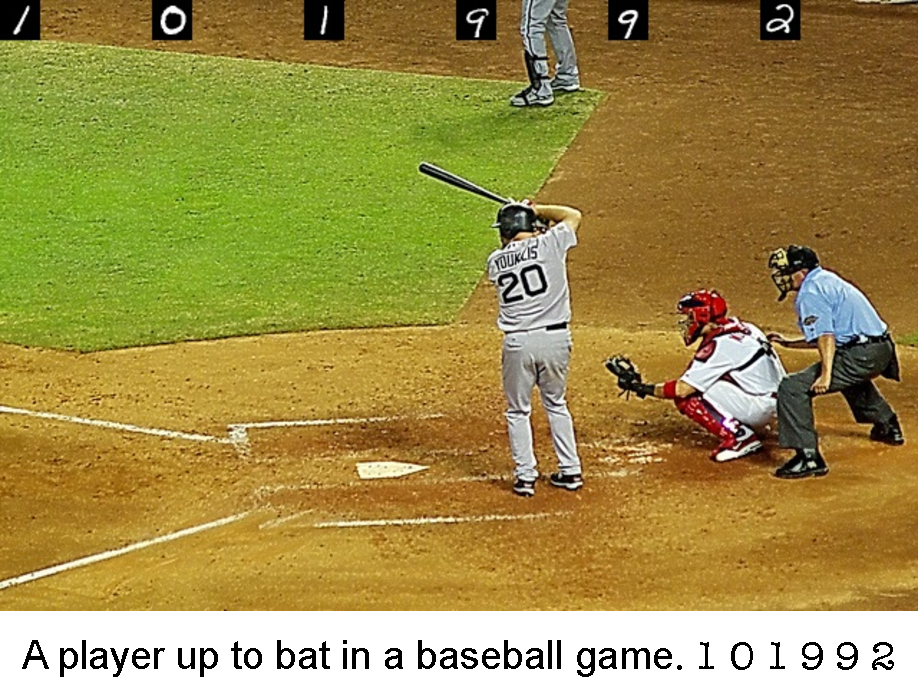
\includegraphics[width=0.4\textwidth]{figures/shortcut-example}
	\caption{An image-caption pair from the MS-COCO dataset with a shortcut added to both the image and the caption.}
	\label{fig:shortcut-example}
\end{wrapfigure}

\header{Synthetic Shortcuts}
In this section, we introduce the \textit{\acf{SVL}} training and evaluation framework.
We denote the \textit{synthetic shortcuts for image-caption data} as $\sct{}$.
The purpose of the framework is to introduce additional and easily identifiable information shared between an image and the matching captions that lacks any semantic meaning. 
The shortcuts we use in this work are represented as numbers that we add to images and captions.
For images, we add the shortcut number by adding MNIST images as an overlay to the original images.
For captions, we append the numbers of the shortcut as extra tokens at the end of the caption.

Figure~\ref{fig:shortcut-example} illustrates an example of an image-caption pair with an added shortcut.
The example contains an image with the caption: `A player up to bat in a baseball game. 1 0 1 9 9 2.'
Here, `1 0 1 9 9 2' is a shortcut added to both the image and the caption. 
For the image modality, we add the shortcut by overlaying MNIST images at the top of the original image.
For the text modality, we append the shortcut as additional tokens at the end of the caption.
This identifier provides an additional link between the image and the caption without carrying any semantic meaning related to their content. 
Additional examples are shown in Figure~\ref{fig:shortcut_examples}.

If contrastive losses learn task-optimal representations, then the presence of synthetic shortcuts should not negatively impact the evaluation performance, since synthetic shortcuts represent additional information and the remaining task-relevant information is intact.
By incorporating synthetic shortcuts into the image-caption dataset, the shared information would include the information that was originally shared and the synthetic shortcut:
$S^{+} = S + \sct{}$.
Hence, the task-relevant information would comprise caption-specific information that was originally shared and a synthetic shortcut:
$R^{+} = C_A + C_B + S + \sct{}$. 
If injecting a synthetic shortcut influences the performance negatively, we can conclude that by learning to represent a synthetic shortcut the model suppresses other task-relevant information in favor of the shortcut, hence the representation is not task-optimal.
The setup is inspired by the ``datasets with explicit and controllable competing features,'' introduced by \cite{chen2021intriguing}, but we adapt this setup to the \ac{VL} scenario.

For experiments, we use the \ac{Flickr30k} and \ac{MS-COCO} image-caption datasets, that consist of image-caption tuples, each image is associated with five captions.
During training, we sample a batch of image-caption pairs $\mathcal{B} = \{(\img{i}, \capt{i}{j}), \dots\}_{i=1}^{|\mathcal{B}|}$, from dataset $\mathcal{D}$, and apply shortcut sampling.
We inject the shortcuts in a manner that preserves the original information of the images and captions. 
Furthermore, we append the shortcut after applying data augmentations to ensure that the shortcut is present in both the images and captions (i.e., the shortcut is not augmented away).
We refer to Figure~\ref{fig:shortcut_examples} for some examples.
The training, evaluation, and implementation details of the shortcut sampling are provided in Appendix~\ref{app:experimental-shortcutsampling}.

We define the following experimental setups:
\begin{enumerate}[label=\Roman*]
	\item \emph{No shortcuts}: As a baseline, we fine-tune a pre-trained CLIP~\citep{radford2021learning} and train VSE++~\citep{faghri2018improving} from scratch on \ac{Flickr30k} and \ac{MS-COCO}, without using any shortcuts. 
	The experimental setup for training both models is provided in Appendix~\ref{app:experimental-models} and \ref{app:experimental-training}. 
	The goal of this setup is to show the retrieval evaluation performance without adding any shortcuts for both a large-scale pre-trained foundation model and a small-scale model trained from scratch.
	\item \emph{Unique shortcuts}: We add a unique shortcut to each image-caption tuple $i \in\mathcal{D}$ in the dataset. 
	In this setup, each image caption pair can be uniquely matched during training by only detecting the shortcut. 
	For each tuple $i \in \mathcal{D}$, we use the number $i$ as the number of the shortcut we inject to the image and captions in the tuple.
	If the contrastive loss learns task-optimal representations, the downstream evaluation performance should not decrease when training with unique shortcuts.
	\item \emph{Unique shortcuts on only one modality}: To show that the shortcuts do not interfere with the original task-relevant information ($S, C_A$, and $C_B$) of the images and captions, we create a dataset with only shortcuts on either the image or caption modality. Therefore, the shortcut cannot be used by the encoders to match an image-caption pair. 
	Hence, we expect the encoders to ignore the shortcuts and extract the features from the original data similar to the features learned by the baseline models in experimental setup \rom{1}.
	\item \emph{N bits of shortcuts}: In this setup, for each image-caption pair in the training batch $\mathcal{B}$, we randomly sample a shortcut number from the range $[0, 2^{n}]$, where $n$ is the number of bits.
	The higher the value of $n$, the more image-caption pairs in the training batch will have by expectation a unique shortcut, and, the less the model has to rely on $S$ and the remaining task-relevant information to solve the contrastive objective. 
	The goal of this setup is to show that, the more unique (shortcut) information is present per sample in the batch, the less contrastive models rely on the remaining task-relevant information.
\end{enumerate}
 It should be noted that the shortcuts we add are independent of the image-caption pairs. 
 However, the goal of the \ac{SVL} framework is to measure the effect of the presence of additional easy-to-detect shared information on the learned representations. 

 \header{Evaluation Method}
To show the effect of the injected shortcuts on retrieval evaluation performance, we evaluate both with and without adding the shortcuts during evaluation.
When training with unique shortcuts, we add a unique shortcut to each tuple in the test set as well.
When training with shortcuts on either one of the two modalities, we only evaluate without shortcuts to show that training with shortcuts on one modality does not influence performance.
When training with $n$ bits of shortcuts, we add the shortcut $\mod(i, n)$ (modulo) to each tuple $i$ in the evaluation set, to make sure we use the same number of shortcuts during evaluation as during training.
To facilitate the reproducibility and support further research, we provide the code with our paper.\footnote{ \url{https://github.com/MauritsBleeker/svl-framework}}
